%%%%%%%%%%%%% Subsystem 4 %%%%%%%%%%%%%%%
\clearpage
\subsection{Subsystem 4: Network and Communications}

% Subsystem Diagram
\subsubsection{Subsystem Diagrams}
\begin{figure}[h]
    \centering
    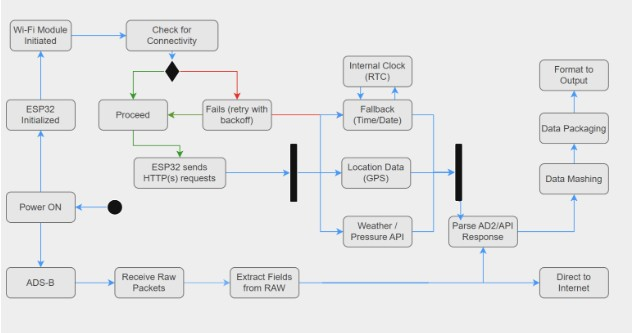
\includegraphics[width=16cm]{images/Communications/SubsystemDiagram-communcations.jpg} % Change the picture
    \caption{Network subsystem Block Diagram}
\end{figure} % If your subsystem is more coding, change it to activity diagram

% Specifications
\subsubsection{Specifications}
\begin{enumerate}
    \item Connection to WPA2 network established in less than 10 s.
    \item HTTPS request latency less than 500 ms for payloads up to 2 kB.
    \item Outbound HTTP POST/GET success rate at least 95\%.
    \item Fallback mode automatically activates within 5 s if there is no connectivity.
    \item Error handling: up to 3 retries with exponential back-off before fallback.
    \item System connectivity uptime at least 95\% during a continuous 1-hour runtime.
    \item Operates at 1090 MHz Extended Squitter (1090ES) frame format.
    \item Reception rate at least 100 packets/s when aircraft are in range.
    \item Typical data rate: around 1000 ADS-B frames per second (raw stream).
    \item Range: at least 200 nautical miles (line-of-sight).
    \item Latency: less than 100 ms for frame decoding.
    \item Error rate: less than 1\% decode errors with comprehensive error logging.
    \item Provides 1Hz fix rate for accurate localization.
    \item Supplies location and time data to synchronize ADS-B and API results.
\end{enumerate}

% Subsystem Interactions
\subsubsection{Subsystem Interactions}
The communications subsystem acts as the Aviator’s data bridge between external information sources and the internal electronics. 
It collects ADS-B, API-airport data, and weather data, then forwards validated information to the Processing Subsystem via serial or SPI communication for formatting and display output.
\newline
Power is provided by the Power Management Subsystem through a regulated 3.3 V rail, ensuring stable operation of the ESP32 and SDR receiver. In return, the communications unit reports basic voltage or connection status when required.
\newline
Externally, this subsystem interacts with aircraft transponders (ADS-B at 1090 MHz), the Open-Meteo API through HTTPS, and other APIs for airport information. 
Combined, these links guarantee the Aviator always has synchronized flight and environmental data for visualization on the display subsystem.


% Core ECE
\subsubsection{Core ECE Design Tasks}
\begin{itemize}
    \item \textbf{ECE 36200}: Programming the ESP32 for SPI/UART communication and Wi-Fi control, configuring serial buses (UART, SPI), and managing real-time I/O between Wi-Fi, GPS, and ADS-B modules.
    \item \textbf{ECE 43800}: Understanding ADS-B packet decoding and signal validation, including digital filtering, sampling, and signal integrity techniques used during packet extraction.
    \item \textbf{ECE 54700}: Provided with a quantitative understanding of network protocols, error recovery, congestion control, and routing, which directly inform the subsystem’s retry logic, exponential back-off, and HTTP/TCP communication design.
    \item \textbf{ECE 20875}: Implementing data parsing and JSON handling for API responses, plus everything in regard to how to code the process in python.
\end{itemize}

% Schematics
\subsubsection{Schematics}
[Type here \textbf{DD2+}]
\begin{figure}[h]
    \centering
    
\includegraphics[width=16cm]{images/white.png} % Change the picture
    \caption{[Schematic Name]}
\end{figure} % If your subsystem is more coding, change it to psudo code

% Parts List
\subsubsection{Parts}
\begin{itemize}
    \item ADS-B Receiver (1090 MHz SDR Dongle): Captures live aircraft broadcast signals (position, altitude, velocity, ICAO ID) using Automatic Dependent Surveillance–Broadcast (ADS-B). Interfaces with the ESP32 via UART or USB-serial bridge
    \item Weather API Module: Software interface for retrieving real-time weather conditions (temperature, wind, pressure, etc.) through HTTPS requests to the Open-Meteo API.
    \item Wi-Fi Network Interface (ESP32 Integrated): Enables wireless internet connectivity for API calls, data uploads, and synchronization with external services. Supports WPA2 and TCP/IP stack.
    \item Data/Signal Interface: Internal software and pathways responsible for merging ADS-B, GPS, and API data. Manages data transfer to the Processing Subsystem via SPI or serial communication
    \item GPS/Geolocation Unit (NEO-6M if used): Provides precise latitude, longitude, and time data at 1 Hz. Used for correlating aircraft positions and providing fallback localization when ADS-B data are unavailable.
\end{itemize}

% Algorithm
\subsubsection{Algorithm}
This Subsystem operates through a multi-threaded architecture that concurrently handles ADS-B signal processing and weather data acquisition, ensuring continuous data availability and synchronization between local and online sources.
\newline
\textbf{ADS-B Processing Pipeline}
\begin{enumerate}   
    \item Signal Acquisition: Continuously monitors the 1090 MHz frequency band for Extended Squitter (DF17) transmissions from aircraft transponders.
    \item Frame Validation: Each 112-bit frame undergoes length verification and CRC-24 checksum validation to ensure data integrity.
    \item Message Classification: Extract the Type Code (TC) from bits 32–37 to determine message content:
    \begin{enumerate}
        \item TC 1–4 → Aircraft identification containing 8-character callsign.
        \item TC 9–18 → Airborne position with barometric altitude and encoded latitude/longitude.
        \item TC 19 → Velocity vectors providing ground speed and track heading.
    \end{enumerate}
    \item Position Decoding: For location messages, implement the Compact Position Reporting (CPR) algorithm, requiring even/odd frame pairs per aircraft to resolve global coordinates.
    \item Database Management: Maintain active flight records indexed by ICAO address, updating position, altitude, and velocity as new frames arrive.
\end{enumerate}

\textbf{Weather Integration Process}
\begin{enumerate}
    \item Periodic API Calls: Issue HTTPS requests to the Open-Meteo service every 15 minutes for current atmospheric conditions.
    \item Multi-Level Data: Retrieve both surface weather and upper-atmosphere conditions at pressure levels (850 hPa – 250 hPa) corresponding to aircraft cruising altitudes.
    \item Spatial Correlation: Match weather data to flight positions, providing contextual meteorological information for each tracked aircraft.
\end{enumerate}

\textbf{Flight Database Correlation (Future Enhancement)}
\begin{enumerate}
    \item Callsign Lookup: Match decoded aircraft callsigns with commercial flight-tracking APIs such as FlightAware or OpenSky Network.
    \item Route Information: Correlate ICAO addresses with scheduled flight data to determine origin–destination pairs, delays, and gate assignments.
    \item Enhanced Display: Transform raw aircraft data (position, altitude) into meaningful flight information (route, delay status, aircraft type).
\end{enumerate}

\textbf{Data Fusion and Export}
\begin{enumerate}
    \item Distance Calculation: Apply the formulas required to compute aircraft proximity to the receiver’s GPS location.
    \item Error Handling: Implement comprehensive logging and retry mechanisms for malformed frames, failed API calls, and decoding errors.
    \item Interface Abstraction: Export processed data through high-level APIs from functions that fetch flight-weather info that encapsulate protocol complexity from downstream subsystems.
\end{enumerate}
Real-Time Operation: Maintaining a continuous operation via non-blocking frame processing, periodic weather updates, automatic database pruning of stale aircraft records, and dual-mode functionality. This will ensure reliable data flow even during bad network or RF interference.
% Theory of Operation
\subsubsection{Theory of Operation}
Upon initialization, the ESP32 microcontroller establishes WiFi connectivity and begins continuous monitoring of the 1090 MHz ADS-B frequency band. 
The ADS-B receiver captures 112-bit Extended Squitter (DF17) frames broadcast by aircraft transponders, containing encoded ICAO identifiers, position data, altitude, and velocity information. 
Each frame undergoes CRC validation and bit-level decoding, extracting Type Codes for identification (TC 1-4), airborne position (TC 9-18), and velocity (TC 19). 
Position data uses Compact Position Reporting (CPR) algorithms, requiring even/odd frame pairs to decode latitude/longitude coordinates.
\newline
Simultaneously, the system issues periodic HTTPS requests to the Open-Meteo weather API, retrieving both surface conditions and upper-atmosphere data at pressure levels (850hPa to 250hPa) corresponding to aircraft cruising altitudes. 
Weather data is correlated with flight positions to provide contextual information. 
Additionally, information from airport information is looked for to match with ADS-B information about planes caught by the antenna, meaning one can match data and determine if flights are delayed, origin-destination, etc.
\newline
The ESP32 processes all incoming data streams in real-time, maintaining an active flight database indexed by ICAO address. 
Distance calculations use formulas to determine aircraft proximity to the receiver. 
Comprehensive error handling includes frame validation, API timeout recovery, and statistical error tracking to ensure robust operation.


% Specification Measurement
\subsubsection{Specifications Measurement}
[\textbf{DD3+} Every specification here should match the specification above. ]
\begin{enumerate}
    \item {[Copy specification here. ]} \\
          {[Explain the specification here. Add photos if necessary. ]}
\end{enumerate}

% Standards
\subsubsection{Standards}
\begin{itemize}
    \item \textbf{NMEA 0183}: Used by GPS receivers to format location/time data, ensuring compatibility with processing algorithms.
    \item \textbf{REST/HTTPS}: Secure, standardized communication with weather servers and external data sources.
    \item \textbf{IEEE 802.11 (Wi-Fi) / IEEE 802.3 (Ethernet)}: Provides reliable networking for internet-based data exchange (when we add website interference).
    \item \textbf{TCP/IP, Checksum validation}: Ensures robustness in communication so that even non-technical users get accurate, reliable results.
\end{itemize}